\documentclass[12pt]{article}

\usepackage{graphicx}
\usepackage{listings}
\usepackage{color}
\usepackage{amsmath}
\usepackage{hyperref}


\begin{document}

\title{Proyecto Base de Datos 1 \\
       \large Autoland}

\author{Lucas Carranza 202210073 \and
        David Herencia 202210408 \and
        Francisco Calle 202210065}

\date{2023}
\begin{figure}
\centering

\includegraphics[width=0.5\textwidth]{autoland.jpeg}
\end{figure}


\maketitle


\begin{center} 

    \noindent Docente: Docente: Chambilla Aquino, Teófilo
    
    \noindent Curso: Base de Datos I
    
    \noindent Universidad de Ingeniería y Tecnología

\end{center}

\newpage

\tableofcontents

\newpage

\section{Requisitos}

\subsection{Introducci\'on}

En este proyecto se desea desarrollar una base de datos para una tienda de autos que se dedica a la compra de vehículos de otras empresas, nuevos y seminuevos, para revenderlos al público. Se basa en la base de datos para la tienda de autos "Autoland" y tiene como objetivo ofrecer vehículos asequibles para el peruano promedio. Debido a la naturaleza de constante rotación de mercancía es necesario modelar una base de datos robusta que permita la entrada de los vehículos adquiridos y la fácil y eficiente consulta de aquellos que están en stock. 

\subsection{Descripci\'on general del problema/organizaci\'on/empresa}

La necesidad de vehículos motorizados es importante en la ciudad de Lima, ya que el transporte público no está muy desarrollado. La tienda de autos busca solucionar esta necesidad ofreciendo vehículos nuevos y seminuevos a precios accesibles, al obtenerlos en suministros de gran cantidad directamente de diversas empresas distribuidoras de vehiculos, o que venden sus flotas usadas de trabajo.

El problema recae en el monitoreo y manejo de la información de esta gran cantidad de vehiculos que rota constantemente en el stock de la tienda. Al usar métodos tradicionales como registros a mano, se requiere mucho tiempo al realizar la compra y venta de vehículos, es difícil para el cliente saber qué tiene la tienda a la venta, existe la posibilidad de error en la lectura y escritura, y se pierde la posibilidad de análisis estadístico de las ventas de la empresa (para obtener un mayor márgen de ganancia/más ventas).

\subsection{Necesidad/usos de la base de datos}

La base de datos es necesaria para llevar un control de los vehículos que se compran, se venden y los que se encuentran en inventario, así como también para llevar un registro de los clientes, los asesores de venta y los representantes.

\subsection{¿Cómo resuelve el problema de hoy?}

La tienda actualmente lleva un registro manual de los vehículos, los clientes y las ventas, lo cual es un proceso lento y propenso a errores. La base de datos ayudará a mejorar el proceso de registro y seguimiento de los vehículos, clientes y ventas. La implementación de la base de datos en la tienda es la solución.

\subsubsection{¿Cómo se almacenan/procesan los datos hoy?}

Actualmente los datos se almacenan en archivos físicos (papel) y en hojas de cálculo en línea (Excel). No hay una base de datos centralizada y el proceso de registro de los vehículos, clientes y ventas se hace manualmente. La consulta de datos se hace igualmente de forma manual.

\subsubsection{Flujo de datos}

El flujo de datos en la base de datos de la tienda va de acorde principalmente con la entrada de vehículos al inventario de esta, así como con la salida al haber ventas. Aquí se describe detalladamente el proceso:

El flujo de datos actual comienza con el suministro de vehículos realizado por parte de los representantes, seguido de la recepción de los vehículos por parte de la tienda. En caso de que el modelo o motor del vehículo no estén registrados, se tienen que añadir previamente a las tablas correspondientes. Durante la estadía en la tienda, los vehículos son inspeccionados una o más veces por los mecánicos, y se registra la participación de cada uno. A continuación, los vehículos son agregados al inventario de la tienda. Los clientes consultan el inventario y realizan compras, supervisadas por los asesores de ventas. Por último, la orden de compra es registrada y el vehiculo deja de ser mostrado en el inventario de la tienda. Los clientes pueden consultar el historial de compras que han realizado ellos.

Igualmente, tras haber realizado una compra, un cliente puede continuar accediendo a servicios de postventa a la tienda, donde se registra cada uno de los servicios al que acude, y la participación de cada mecánico en estos.

\subsection{Descripci\'on detallada del sistema}

\subsubsection{Objetivos de información actuales}

Los objetivos de información actuales son llevar un control de los vehículos en inventario y las compras, para así poder tener un sitio web desde el que los clientes pueden realizar compras, consultar la disponibilidad de los modelos de su preferencia, y entre otras acciones para aumentar el alcance y ventas del negocio de Autoland.

Adicionalmente, tener un control con una base de datos permitirá realizar análisis estadísticos de las ventas, para así poder tomar decisiones que aumenten las ventas y el margen de ganancia. Es así como se puede priorizar los modelos más comprados por los clientes, ajustar los precios en función a la demanda, u ofrecer ofertas personalizadas a ciertos clientes tras analizar sus patrones de consumo.

\subsubsection{Caracter\'isticas y funcionalidades esperadas}

Se espera que la base de datos permita llevar un registro de los vehículos en inventario, de los clientes y de las ventas realizadas. También se espera que permita generar reportes y estadísticas sobre el inventario, las ventas y los clientes.

\subsubsection{Tipos de usuarios existentes/necesarios}

Los tipos de usuarios necesarios son los asesores de ventas, los clientes y los representantes. Se espera que el representante brinde la información requerida de cada vehículo suministrado, la cual será incorporada en la base de datos. Así se elimina la necesidad de añadir manualmente con un administrador.

\subsubsection{Tipos de consulta, actualizaciones}

Los tipos de consulta y actualización que se esperan por parte de los clientes son: Consulta del stock (vehículos),  consulta de las compras realizadas. Actualización (Eliminar/ocultar) la lista de vehículos al realizar la compra, registro de la compra.

Se registra la lista de vehículos añadida al realizar un suministro. Igualmente, se registra el motor y modelo cuando se añaden vehículos con estos no presentes en la base de datos.

Las consultas esperadas son consultas de inventario, consultas de clientes y consultas de ventas realizadas. Las actualizaciones que se esperan son actualizaciones de inventario, actualizaciones de clientes y actualizaciones de ventas realizadas.


\subsubsection{Tama\~no de la base de datos}

El tamaño de la base de datos es directamente proporcional al tamaño del negocio, así como la frecuencia de las ventas. El tamaño del negocion nos da una perspectiva de la cantidad de vehículos en stock por vez, y la frecuencia de las ventas nos da una perspectiva de la tasa de crecimiento de las tablas de clientes y compras.

En el caso de autoland, un negocio con 10 locales en todo lima, y un total de unos 300-400 vehículos en stock por vez, estimamos una venta por día, y aproximadamente 360 ventas anuales.

\newpage

\begin{table}[h]
    \centering
    \begin{tabular}{|l|p{4cm}|p{4cm}|}
    \hline
    \textbf{Nombre de la tabla} & \textbf{Longitud de atributo en Bytes} & \textbf{Longitud del registro en Bytes} \\ \hline
    Asesor                      & 8 + 50 + 50 + 11 + 4                  & 123                                    \\ \hline
    Mecánico                    & 8 + 50 + 50 + 11 + 4                  & 123                                    \\ \hline
    Cliente                     & 8 + 50 + 50                           & 108                                    \\ \hline
    representante                   & 8 + 50 + 50 + 11                      & 119                                    \\ \hline
    Empresa                     & 8 + 100                               & 108                                    \\ \hline
    Compra                      & 8 + 4 + 17 + 8 + 4                    & 41                                     \\ \hline
    Suministro                  & 8 + 4 + 4 + 4                         & 20                                     \\ \hline
    Vehículo                    & 17 + 20 + 4 + 4 + 10 + 20 + 4 + 20 + 1 & 100                                    \\ \hline
    Motor                       & 20 + 20 + 20 + 4 + 4 + 4              & 72                                     \\ \hline
    Modelo                      & 4 + 20 + 20 + 4 + 4                   & 52                                     \\ \hline
    ServicioPostVenta           & 8 + 4 + 4 + 15 + 4                    & 35                                     \\ \hline
    m\_inspecciona              & 8 + 17 + 4                            & 29                                     \\ \hline
    m\_trabaja                  & 8 + 4 + 8                             & 20                                     \\ \hline
    \end{tabular}
    \caption{Estimación de la Base de Datos}
\end{table}

\begin{table}[h]
    \centering
    \begin{tabular}{|l|l|l|l|}
    \hline
    \textbf{Nombre de la tabla} & \textbf{Datos estimados anualmente} & \textbf{Tamaño en Bytes} & \textbf{Total anual} \\ \hline
    Asesor                      & 40         & 123 & 4920                                   \\ \hline
    Mecánico                    & 40         & 123 & 4920                                   \\ \hline
    Cliente                     & 320        & 108 & 34560                                  \\ \hline
    representante                   & 60         & 119 & 7140                                   \\ \hline
    Empresa                     & 20         & 108 & 2160                                   \\ \hline
    Compra                      & 360        & 41 & 14760                                 \\ \hline
    Suministro                  & 300        & 20 & 6000                                   \\ \hline
    Vehículo                    & 600        & 100 & 60000                                   \\ \hline
    Motor                       & 75         & 72 & 5400                                    \\ \hline
    Modelo                      & 150        & 52 & 7800                                    \\ \hline
    ServicioPostVenta           & 800        & 35  & 28000                                  \\ \hline
    m\_inspecciona              & 1000       & 29  & 29000                                  \\ \hline
    m\_trabaja                  & 2000       & 20 & 40000                                   \\ \hline
    \end{tabular}
    \caption{Estimación del tamaño tras un año}
\end{table}

\textbf{TOTAL:} 244660 Bytes

\newpage

\subsection{Objetivos del proyecto}

\begin{itemize}

\item El proyecto en cuestion tiene como proposito mejorar la data de Autoland usando conocimientos en bases de datos para lograr un mejor manejo de la información recibida por medio de procesos.

\item Como segundo proposito buscamos mejorar el tiempo de respuesta al momento de solicitar información o ingresarla.

\end{itemize}

\subsection{Referencias del proyecto}

El proyecto se inspiró en tiendas de autos como Autoland, que tienen un gran stock de vehículos y que necesitan llevar un registro de los mismos, así como de los clientes y las ventas realizadas. Originalmente planeamos un portal en línea como neoauto donde se pueden comprar y vender vehículos, pero decidimos que una base de datos para una tienda funcionaría mejor.

\subsection{Eventualidades}

\subsubsection{Problemas que pudieran encontrarse en el proyecto}

Nuestro proyecto cuenta con las siguientes posibles problemas:

\begin{itemize}

\item No se incluye un sistema de autenticación de usuarios, por lo que no se puede distinguir entre los diferentes tipos de usuarios (clientes, asesores de ventas, representantes) cuando se filtre por su llave única (DNI).

\item La base de datos no considera servicios de garantía, por lo que no se puede llevar un registro de los servicios de garantía que se ofrecen a los clientes.

\item Se ha priorizado el entendimiento del modelo por encima de la eficiencia de las consultas, por lo que el tiempo de consultas puede no ser el mejor posible. Aún así, se ha intentado optimizar las consultas para que sean lo más eficientes posibles.

\item No existe la posibilidad de comprar más de un vehículo por compra.

\item No se considera la posibilidad de contratar a empleados extranjeros que no cuenten con DNI. Tampoco la posibilidad de vender a ciudadanos no peruanos o vender directamente a personas jurídicas (empresas).

\item Los clientes no pueden dar su vehículo como parte de pago para la compra de otro vehículo.

\item La tienda no puede obtener vehículos de personas naturales (individuos).

\item No se mantiene un registro de las piezas usadas en el mantenimiento y reparación de los vehículos en los servicios de postventa.

\end{itemize}


\subsubsection{Limites y alcances del proyecto}

\begin{itemize}

\item Alcances

Este proyecto tendrá un alcance a cualquier tienda con un modelo de negocio compatible al de Autoland dentro del país, y se espera que sea usada por una tienda de venta de vehículos como Autoland, la cual cuenta con sedes en diversos distritos de la ciudad de Lima Metropolitana.

\item Limites

Este proyecto no aplica para tiendas de venta de vehículos que no tengan un modelo de negocio compatible, como por ejemplo, tiendas de venta de vehículos de segunda mano que compran a personas naturales en vez de personas jurídicas (empresas). Tampoco considera negocios que lidien con extranjeros, sea al contratarlos como asesores, o al vender a clientes sin documento de identidad nacional (DNI).


\end{itemize}


\section{Modelo Entidad-Relaci\'on}

\subsection{Reglas sem\'anticas}

A continuación, las reglas semánticas que definen el fucionamiento de la base de datos:

\begin{itemize}
\item La tienda contrata asesores de ventas que se encargan de supervisar la venta de vehículos. Cuentan con DNI, RUC, Nombres, Apellidos y Salario.
\item La tienda contrata mecánicos. Cuentan con DNI, RUC, Nombres, Apellidos y Salario. Estos pueden encargarse de realizar inspecciones a vehículos antes de su adquisición por parte de la tienda, o servicios de postventa a los clientes.
\item Los clientes se identifican con su DNI, Nombres y Apellidos. Para ser considerado cliente, debe haber realizado por lo menos una compra.
\item Los representantes son los agentes que se encargan de representar a las compañías que nos suministran de vehículos (por política de la tienda, no se lidia con las empresas directamente). Se identifican con su DNI. Cuentan con nombres y apellidos. Cada representante trabaja para una sola empresa, que se identifica con su razón social y RUC.

\item Los clientes pueden realizar múltiples compras.
\item La compra de un vehículo debe ser atendida solo por un asesor de ventas, y se registra con un código numérico único, y la fecha en la que se realizó.
\item Cada compra corresponde a la adquisición de un solo vehículo.

\item Un cliente tiene la posibilidad de acceder a cero o más servicios de postventa. Este servicio sólo está disponible si el cliente ha realizado una compra.
\item El servicio de postventa se identifica con el número de orden en el que se realizó. Además, se registra la fecha de inicio y fin, el tipo de servicio (reparación, mantenimiento, pintura) y el costo.
\item Múltiples mecánicos pueden trabajar en un servicio de postventa. Cada fecha que un mecánico trabaja en uno se registra, junto con el costo del material usado en el servicio para ese día.

\item Los representantes realizan suministros. Para ser registrado como representante debe haber realizado mínimo un suministro a la tienda.
\item Cada suministro corresponde a un solo representante.
\item Cada suministro añade uno o más vehículos al inventario de nuestra empresa.
\item Cada suministro se identifica con un código numérico. Además incluye la fecha en la que se realizó.

\item Tenemos vehículos cuyo identificador único es el código alfanumérico VIN.
\item Los vehículos cuentan con el color de pintura y precio de venta.
\item Los vehículos, si son usados, tienen kilometraje. Si son nuevos, este será 0.
\item Se registra el precio al que se compró el vehículo, y el precio al que se venderá a los clientes.

\item Todos los vehículos son inspeccionados por lo menos una vez por uno o más mecánicos, se registra la fecha de inspección y se identifica con el número de esta.
\item Cada inspección corresponde a un vehículo. Cada vehículo puede ser inspeccionado múltiples veces de ser necesario.

\item Todos los vehículos cuentan con una transmisión.
\item La transmisión puede ser de 3 tipos: automática, manual o secuencial.

\item Los vehículos cuentan con un solo motor. Un tipo de motor puede encontrarse en muchos vehículos, o igualmente, en ninguno.
\item El motor se identifica por su código alfanumérico correspondiente a su modelo. Además se identifica por su marca, tipo de combustible, número de cilindros, cilindrada, y finalmente, la potencia.

\item Cada vehículo corresponde a exactamente un Modelo.
\item Todos los modelos se identifican por su ID numérico único, además tienen Marca, Nombre, Año y Precio Sugerido.
\item Hay 4 categorías de Modelo: auto, camioneta, moto y camión.
\end{itemize}

\subsection{Modelo Entidad-Relaci\'on}

A continuación, el modelo entidad-relación que representa a la base de datos:

\begin{figure}
\centering
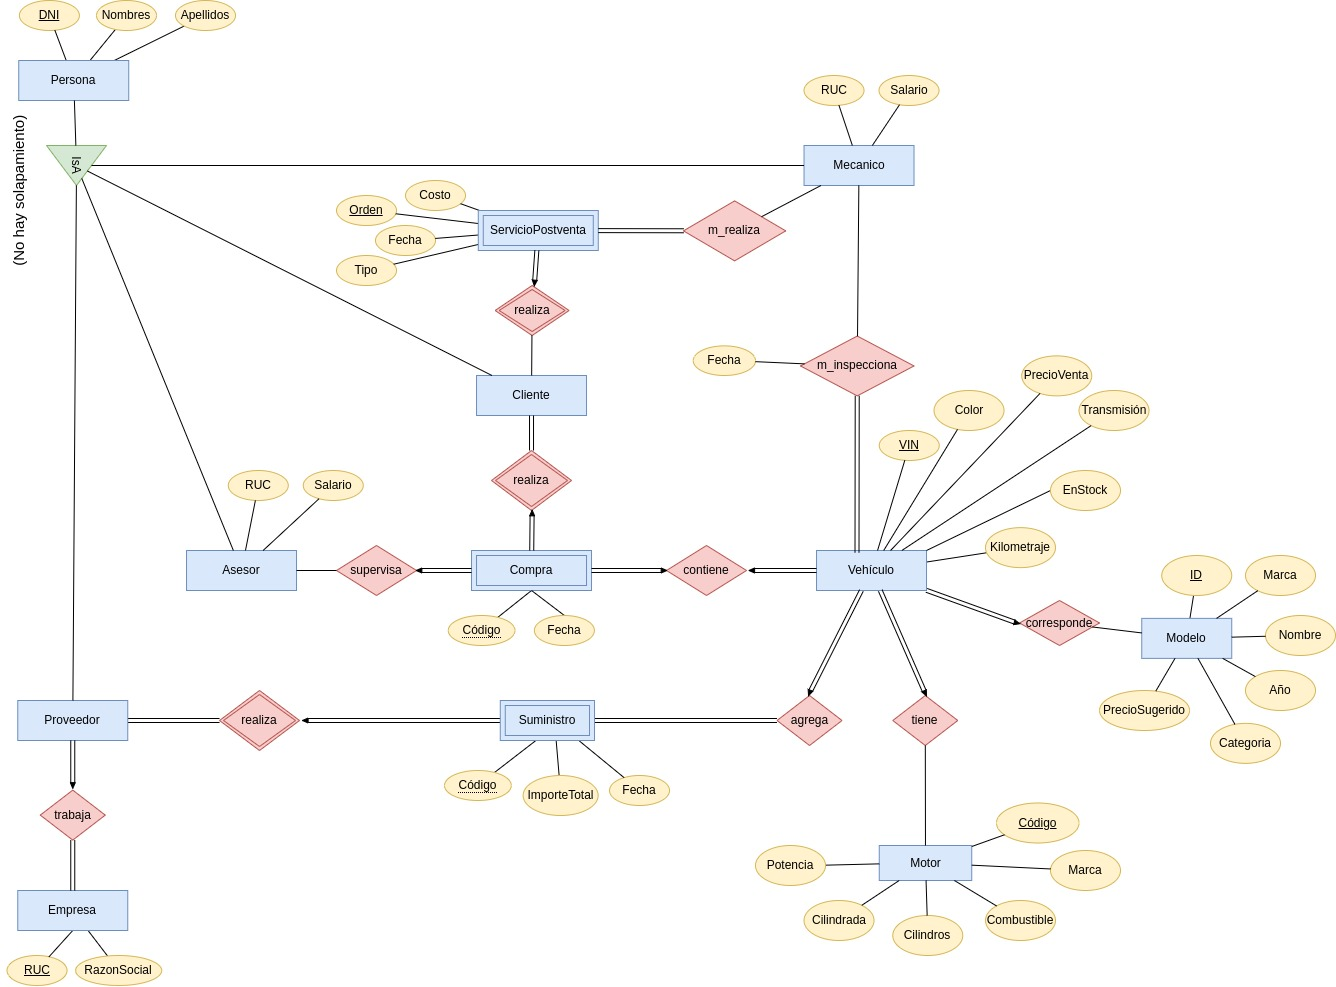
\includegraphics[width=1\textwidth]{ER.jpg}
\caption{Modelo Entidad-Relación}
\end{figure}

\subsection{Especificaciones y consideraciones sobre el modelo}

\subsubsection{Entidad Persona}
\textbf{Especificaciones}

Clase padre de Cliente, Asesor, Mecánico y representante. Contiene la información necesaria para identificarlos como sus Nombres y Apellidos, y su llave primaria es el DNI.

\textbf{Consideraciones}

Se usa el DNI como llave primaria por la posibilidad de homonimia y la facilidad que este provee como identificador único.

\subsubsection{Entidad Cliente}
\textbf{Especificaciones}

Subclase de Persona usada para los Clientes, no contiene atributos adicionales, pues no se solicitan datos adicionales sobre el cliente. Su llave primaria es el DNI.

\textbf{Consideraciones}

Un cliente puede realizar múltiples compras y acceder a múltiples servicios de postventa, por lo que se establece una relación entre las entidades Cliente, Compra y ServicioPostVenta.

\subsubsection{Entidad Asesor}
\textbf{Especificaciones}

Contiene información específica del asesor, como su Salario y su RUC personal, y su llave primaria es el DNI.

\textbf{Consideraciones}

Un asesor puede atender múltiples compras, por lo que se establece una relación entre las entidades Asesor y Compra. 

\subsubsection{Entidad Mecánico}
\textbf{Especificaciones}

Contiene información específica del mecánico, como su Salario y RUC personal, y su llave primaria es el DNI.

\textbf{Consideraciones}

Un mecánico puede realizar múltiples servicios de postventa, por lo que se establece una relación entre las entidades Mecánico y ServicioPostVenta. Igulamente puede realizar inspecciones a los vehiculos, por lo que se establece la relación con la entidad Inspección, la cual se relaciona con Vehículo, debido a la posibilidad de múltiples inspecciones al mismo vehículo por el mismo mecánico.

\subsubsection{Entidad Representante}
\textbf{Especificaciones}

Subclase de Persona usada para los representantes de las empresas a las que la tienda compra vehículos. No contiene información específica de su clase, y su llave primaria es su nombre.

\textbf{Consideraciones}

Un representante puede proveer múltiples suministros, por lo que se establece una relación entre las entidades Representante y Suministro.

\subsubsection{Entidad Empresa}
\textbf{Especificaciones}

Contiene información específica de la empresa, como su Razón Social, y su llave primaria es su RUC de empresa.

\textbf{Consideraciones}

Una empresa puede tener múltiples empleados que son representantes a nuestra tienda, por lo que se establece una relación entre las entidades Empresa, representante. Su RUC es único por lo que se utiliza convenientemente como clave primaria.

\subsubsection{Entidad Suministro}
\textbf{Especificaciones}

Contiene información específica del suministro realizado por un representante, como la fecha en la que se realizó. Su llave primaria es código numérico asignado. Absorbe como llave foránea el DNI del representante.

\textbf{Consideraciones}

Un suministro puede incluir múltiples vehículos, por lo que se establece una relación entre las entidades Suministro y Vehículo. El código numérico es asignado de manera ordenada y no se repite.

\subsubsection{Entidad Compra}
\textbf{Especificaciones}

Contiene información específica de la compra, como la fecha en la que se realizó. Su llave primaria es el código numérico. Absorbe como llaves foráneas el DNI del cliente y el VIN del vehículo comprado.

\textbf{Consideraciones}

Compra es una relación débil de Cliente, pues no existe sin este. Una compra incluye solamente un vehículo, por lo que se establece la relación 1 a 1 entre Compra y Vehículo. Se obtiene como llave foránea al VIN del vehículo. El código numérico es asignado de manera ordenada y no se repite.

\subsubsection{Entidad Vehículo}
\textbf{Especificaciones}

Contiene información específica de cada vehículo que ha pasado por la tienda. Se almacena su marca, modelo, tipo de transmisión, color, precio, kilometraje, su precio de compra en el suministro, y su precio para la venta. Recibe como llaves foráneas al código de su motor y el id del modelo, así como el cóðigo del suministro con el que se obtuvo. Su llave primaria es su código VIN.

\textbf{Consideraciones}

Se utiliza el código VIN pues es un número único asignado a cada vehículo al ser fabricado. Un vehículo que pertenece a la tabla solo puede ser comprado si se encuentra en stock, por lo que se establece una relación entre las entidades Vehículo y Compra. El vehículo es añadido a la tabla a través de un suministro, por lo que se establece la relación entre Vehículo y Suministro. Los vehículos son inspeccionados antes de ser agregados por uno o más mecánicos, por lo que se establece la relación entre Mecánico y Vehículo.


\subsubsection{Entidad Modelo}
\textbf{Especificaciones}

Contiene información específica de cada modelo de vehículo relevante a la tienda. Se almacena su marca, nombre, año y precio sugerido. Su llave primaria es su id numérico asignado por la tienda.

\textbf{Consideraciones}

Se utiliza un id numérico pues es más fácil de manejar que el nombre del modelo. Un modelo puede tener múltiples vehículos, por lo que se establece una relación entre las entidades Modelo y Vehículo.

\subsubsection{Entidad ServicioPostVenta}
\textbf{Especificaciones}

Contiene información específica de cada servicio de postventa. Se almacena la fecha en la que se realizó, el tipo del servicio, el costo a pagar, la fecha de inicio y la fecha del final. Su llave primaria está conformada por el código de la compra del vehículo en el que se realiza, y el código del orden en el que se realiza.

\textbf{Consideraciones}

Servicio de PostVenta es una entidad débil de Compra, pues no se puede identificar sin el vehículo comprado al que se realiza. Se utiliza el número de orden como llave parcial, pues es un número único asignado a cada servicio de postventa. Un servicio de postventa puede ser realizado por uno o más mecánicos, por lo que se establece una relación entre las entidades ServicioPostVenta y Mecánico, y se registra en que momento trabajaron en este, y cual fue el costo de los insumos utilizados en este día de trabajo.

\section{Modelo Relacional}

\subsection{Modelo Relacional}
\begin{enumerate}
\item Asesor(\textbf{\underline{DNI: VARCHAR(8)}}, Nombres: VARCHAR(50), Apellidos: VARCHAR(50), RUC: VARCHAR(11), Salario: FLOAT)
\item Mecánico(\textbf{\underline{DNI: VARCHAR(8)}}, Nombres: VARCHAR(50), Apellidos: VARCHAR(50), RUC: VARCHAR(11), Salario: FLOAT)
\item Cliente(\textbf{\underline{DNI: VARCHAR(8)}}, Nombres: VARCHAR(50), Apellidos: VARCHAR(50))
\item representante(\textbf{\underline{DNI: VARCHAR(8)}}, Nombres: VARCHAR(50), Apellidos: VARCHAR(50), Empresa.RUC: VARCHAR(11))
\item Empresa(\textbf{\underline{RUC: VARCHAR(8)}}, RazonSocial: VARCHAR(100))
\item Compra(\textbf{\underline{Cliente.DNI: VARCHAR(8)}, \underline{Código: INT}}, Vehículo.VIN:, Asesor.DNI, Fecha: DATE)
\item Suministro(\textbf{\underline{representante.DNI: VARCHAR(8)}, \underline{Código: INT}}, Fecha: DATE, Importe: FLOAT)
\item Vehículo(\textbf{\underline{VIN: VARCHAR(17)}}, Color: VARCHAR(20), Precio: FLOAT, Kilometraje: INT, Transmisión: VARCHAR(10), EnStock: BOOLEAN, Motor.Código: VARCHAR(20), Modelo.ID: INT, Modelo.Categoria: VARCHAR(20))
\item Motor(\textbf{\underline{Código: VARCHAR(20)}}, Marca: VARCHAR(20), Combustible: VARCHAR(20), Cilindros: INT, Cilindrada: INT, Potencia: INT)
\item Modelo(\textbf{\underline{ID: INT}}, Marca: VARCHAR(20), Nombre: VARCHAR(20), Año: INT, PrecioSugerido: FLOAT)
\item ServicioPostventa(\textbf{\underline{Cliente.DNI: VARCHAR(8)}, \underline{Orden: INT}}, Fecha: DATE, Tipo : VARCHAR(15), Costo: FLOAT)
\item m\_inspecciona(\textbf{\underline{Mecanico.DNI: VARCHAR(8)}, \underline{Vehiculo.VIN: VARCHAR(17)}}, Fecha: DATE)
\item m\_trabaja(\textbf{\underline{Mecanico.DNI: VARCHAR(8)}, \underline{ServicioPostventa.Orden: INT}}, \underline{Cliente.DNI: VARCHAR(8)})
\end{enumerate}

\newpage

\subsection{Especificaciones de transformaci\'on}

\subsubsection{Entidades}


\begin{table}[htbp]
\begin{center}
\begin{tabular}{|c|c|}
\hline
Tabla & Empresa \\
\hline
Clave Primaria & RUC \\
\hline
Clave Foránea & N/A \\
\hline
\end{tabular}
\caption{Tabla Empresa}
\end{center}
\end{table}


\begin{table}[htbp]
\begin{center}
\begin{tabular}{|c|c|}
\hline
Tabla & Vehículo \\
\hline
Clave Primaria & VIN \\
\hline
Clave Foránea & Motor.Código, Modelo.ID \\
\hline
\end{tabular}
\caption{Tabla Vehículo}
\end{center}
\end{table}


\begin{table}[htbp]
\begin{center}
\begin{tabular}{|c|c|}
\hline
Tabla & Motor \\
\hline
Clave Primaria & Código \\
\hline
Clave Foránea & N/A \\
\hline
\end{tabular}
\caption{Tabla Motor}
\end{center}
\end{table}


\begin{table}[htbp]
\begin{center}
\begin{tabular}{|c|c|}
\hline
Tabla & Modelo \\
\hline
Clave Primaria & ID \\
\hline
Clave Foránea & N/A \\
\hline
\end{tabular}
\caption{Tabla Modelo}
\end{center}
\end{table}

\newpage

\subsubsection{Entidades d\'ebiles}

\begin{table}[htbp]
\begin{center}
\begin{tabular}{|c|c|}
\hline
Tabla & Compra \\
\hline
Entidad Débil & Compra \\
\hline
Entidad Fuerte & Cliente \\
\hline
Clave Primaria & Cliente.DNI, Código \\
\hline
Clave Foránea & Cliente.DNI, Asesor.DNI, Vehículo.VIN \\
\hline
\end{tabular}
\caption{Tabla Compra}
\end{center}
\end{table}


\begin{table}[htbp]
\begin{center}
\begin{tabular}{|c|c|}
\hline
Tabla & Suministro \\
\hline
Entidad Débil & Suministro \\
\hline
Entidad Fuerte & Cliente \\
\hline
Clave Primaria & Representante.DNI, Código \\
\hline
Clave Foránea & Representante.DNI \\
\hline
\end{tabular}
\caption{Tabla Suministro}
\end{center}
\end{table}


\begin{table}[htbp]
\begin{center}
\begin{tabular}{|c|c|}
\hline
Tabla & ServicioPostVenta \\
\hline
Entidad Débil & ServicioPostVenta \\
\hline
Entidad Fuerte & Cliente \\
\hline
Clave Primaria & Cliente.DNI, Orden \\
\hline
Clave Foránea & Cliente.DNI \\
\hline
\end{tabular}
\caption{Tabla ServicioPostventa}
\end{center}
\end{table}

\newpage

\subsubsection{Entidades superclase/subclase}

\begin{table}[htbp]
\begin{center}
\begin{tabular}{|c|c|}
\hline
Tabla & Persona \\
\hline
Entidad Superclase & Persona \\
\hline
Entidad Subclase & Cliente, Mecánico, Asesor, Representante \\
\hline
Clave Primaria & DNI \\
\hline
Clave Foránea & N/A \\
\hline
\end{tabular}        
\caption{Tabla Persona}
\end{center}
\end{table}

\newpage

\subsubsection{Relaciones binarias}

\begin{table}[htbp]
\begin{center}
\begin{tabular}{|c|c|}
\hline
Tabla & m\_inspecciona \\
\hline
Clave Primaria & Mecánico.DNI, Vehículo.VIN \\
\hline
Clave Foránea & Mecánico.DNI, Vehículo.VIN \\
\hline
\end{tabular}
\caption{Tabla m\_inspecciona}
\end{center}
\end{table}

\begin{table}[htbp]
\begin{center}
\begin{tabular}{|c|c|}
\hline
Tabla & m\_trabaja \\
\hline
Clave Primaria & Mecánico.DNI, ServicioPostVenta.Orden, Cliente.DNI \\
\hline
Clave Foránea & Mecánico.DNI, ServicioPostVenta.Orden, Cliente.DNI \\
\hline
\end{tabular}
\caption{Tabla m\_inspecciona}
\end{center}
\end{table}

\newpage

\subsection{Diccionario de datos}

\begin{table}[htbp]
    \begin{center}
    \begin{tabular}{|p{3cm}|p{3cm}|p{1cm}|p{1cm}|p{6cm}|}
        \hline
        Nombre Campo & Tipo de dato & PK & FK & Descripción \\
        \hline
        DNI & VARCHAR(8) & X &  & Número de identificación del asesor \\
        Nombres & VARCHAR(50) &  &  & Nombres del asesor \\
        Apellidos & VARCHAR(50) &  &  & Apellidos del asesor \\
        RUC & VARCHAR(11) &  &  & Registro Único del Contribuyente del asesor \\
        Salario & FLOAT &  &  & Salario del asesor \\
        \hline
        \end{tabular}
        \caption{Tabla Asesor}
            \end{center}
\end{table}


\begin{table}[htbp]
    \begin{center}
        \begin{tabular}{|p{3cm}|p{3cm}|p{1cm}|p{1cm}|p{6cm}|}
            \hline
            Nombre Campo & Tipo de dato & PK & FK & Descripción \\
            \hline
            DNI & VARCHAR(8) & X &  & Número de identificación del mecánico \\
            Nombres & VARCHAR(50) &  &  & Nombres del mecánico \\
            Apellidos & VARCHAR(50) &  &  & Apellidos del mecánico \\
            RUC & VARCHAR(11) &  &  & Registro Único del Contribuyente del mecánico \\
            Salario & FLOAT &  &  & Salario del mecánico \\
            \hline
            \end{tabular}
        \caption{Tabla Mecanico}
            \end{center}
\end{table}


\begin{table}[htbp]
    \begin{center}
        \begin{tabular}{|p{3cm}|p{3cm}|p{1cm}|p{1cm}|p{6cm}|}
            \hline
            Nombre Campo & Tipo de dato & PK & FK & Descripción \\
            \hline
            DNI & VARCHAR(8) & X &  & Número de identificación del cliente \\
            Nombres & VARCHAR(50) &  &  & Nombres del cliente \\
            Apellidos & VARCHAR(50) &  &  & Apellidos del cliente \\
            \hline
            \end{tabular}
        \caption{Tabla Cliente}
            \end{center}
\end{table}


\begin{table}[htbp]
    \begin{center}
        \begin{tabular}{|p{3cm}|p{3cm}|p{1cm}|p{1cm}|p{6cm}|}
            \hline
            Nombre Campo & Tipo de dato & PK & FK & Descripción \\
            \hline
            DNI & VARCHAR(8) & X &  & Número de identificación del representante \\
            Nombres & VARCHAR(50) &  &  & Nombres del representante \\
            Apellidos & VARCHAR(50) &  &  & Apellidos del representante \\
            Empresa.RUC & VARCHAR(11) &  & X & Registro Único del Contribuyente de la empresa representantea \\
            \hline
            \end{tabular}
        \caption{Tabla representante}
            \end{center}
\end{table}


\begin{table}[htbp]
    \begin{center}
        \begin{tabular}{|p{3cm}|p{3cm}|p{1cm}|p{1cm}|p{6cm}|}
            \hline
            Nombre Campo & Tipo de dato & PK & FK & Descripción \\
            \hline
            RUC & VARCHAR(8) & X &  & Registro Único del Contribuyente de la empresa \\
            RazonSocial & VARCHAR(100) &  &  & Razón social de la empresa \\
            \hline
            \end{tabular}
        \caption{Tabla Empresa}
            \end{center}
\end{table}


\begin{table}[htbp]
    \begin{center}
        \begin{tabular}{|p{3cm}|p{3cm}|p{1cm}|p{1cm}|p{6cm}|}
            \hline
            Nombre Campo & Tipo de dato & PK & FK & Descripción \\
            \hline
            Cliente.DNI & VARCHAR(8) & X & X & Documento de identificación del cliente\\
            Código & INT & X &  & Código de la compra \\
            Vehículo.VIN & VARCHAR(17) &  & X & Número de identificación del vehículo comprado \\
            Asesor.DNI & VARCHAR(8) &  & X & Número de identificación del asesor encargado de la venta \\
            Fecha & DATE &  &  & Fecha de la compra \\
            \hline
        \end{tabular}
        \caption{Tabla Compra}
            \end{center}
\end{table}


\begin{table}[htbp]
    \begin{center}
        \begin{tabular}{|p{3cm}|p{3cm}|p{1cm}|p{1cm}|p{6cm}|}
            \hline
            Nombre Campo & Tipo de dato & PK & FK & Descripción \\
            \hline
            Representante.DNI & VARCHAR(8) & X & X & Número de identificación del representante \\
            Código & INT & X &  & Código del suministro \\
            Fecha & DATE &  &  & Fecha del suministro \\
            Importe & FLOAT &  &  & Importe del suministro \\
            \hline
            \end{tabular}
        \caption{Tabla Suministro}
            \end{center}
\end{table}


\begin{table}[htbp]
    \begin{center}
        \begin{tabular}{|p{3cm}|p{3cm}|p{1cm}|p{1cm}|p{6cm}|}
            \hline
            Nombre Campo & Tipo de dato & PK & FK & Descripción \\
            \hline
            VIN & VARCHAR(17) & X &  & Número de identificación del vehículo \\
            Color & VARCHAR(20) &  &  & Color del vehículo \\
            Precio & FLOAT &  &  & Precio del vehículo \\
            Kilometraje & INT &  &  & Kilometraje del vehículo \\
            Transmisión & VARCHAR(10) &  &  & Tipo de transmisión del vehículo \\
            Motor.Código & VARCHAR(20) &  & X & Código del motor del vehículo \\
            Modelo.ID & INT &  & X & ID del modelo del vehículo \\
            Modelo.Categoria & VARCHAR(20) &  & X & Categoría del modelo del vehículo \\
            \hline
            \end{tabular}
        \caption{Tabla Vehiculo}
            \end{center}
\end{table}


\begin{table}[htbp]
    \begin{center}
        \begin{tabular}{|p{3cm}|p{3cm}|p{1cm}|p{1cm}|p{6cm}|}
            \hline
            Nombre Campo & Tipo de dato & PK & FK & Descripción \\
            \hline
            Código & VARCHAR(20) & X &  & Código del motor \\
            Marca & VARCHAR(20) &  &  & Marca del motor \\
            Combustible & VARCHAR(20) &  &  & Tipo de combustible del motor \\
            Cilindros & INT &  &  & Número de cilindros del motor \\
            Cilindrada & INT &  &  & Cilindrada del motor \\
            Potencia & INT &  &  & Potencia del motor \\
            \hline
            \end{tabular}
        \caption{Tabla Motor}
            \end{center}
\end{table}


\begin{table}[htbp]
    \begin{center}
        \begin{tabular}{|p{3cm}|p{3cm}|p{1cm}|p{1cm}|p{6cm}|}
            \hline
            Nombre Campo & Tipo de dato & PK & FK & Descripción \\
            \hline
            ID & INT & X &  & ID del modelo \\
            Marca & VARCHAR(20) &  &  & Marca del modelo \\
            Nombre & VARCHAR(20) &  &  & Nombre del modelo \\
            Año & INT &  &  & Año del modelo \\
            PrecioSugerido & FLOAT &  &  & Precio sugerido del del auto\\
            \hline
        \end{tabular}
        \caption{Tabla Modelo}
            \end{center}
\end{table}


\begin{table}[htbp]
    \begin{center}
        \begin{tabular}{|p{3cm}|p{3cm}|p{1cm}|p{1cm}|p{6cm}|}
            \hline
            Nombre Campo & Tipo de dato & PK & FK & Descripción \\
            \hline
            Cliente.DNI & VARCHAR(8) & X & X & Número de identificación del cliente \\
            Orden & INT & X &  & Número de orden del servicio postventa \\
            Fecha & DATE &  &  & Fecha del servicio postventa \\
            Tipo & VARCHAR(15) &  &  & Tipo de servicio postventa \\
            Costo & FLOAT &  &  & Costo del servicio postventa \\
            \hline
        \end{tabular}
        \caption{Tabla ServicioPostventa}
            \end{center}
\end{table}


\begin{table}[h]
    \begin{center}
        \begin{tabular}{|l|l|}
            \multicolumn{2}{l}{\textbf{m\_trabaja}} \\
            \hline
            Tabla & m\_trabaja \\ \hline        
            Entidades & Mecanico, ServicioPostventa \\ \hline
            Nombre Relación & Realiza \\ \hline
            Atributos Relación &  \\ \hline
            Clave Primaria & Mecanico.DNI, ServicioPostventa.Orden \\ \hline
            Clave Foranea ServicioPostventa & ServicioPostventa.Orden \\ \hline
            Clave Foranea Mecanico & Mecanico.DNI \\
            \hline
            \end{tabular}
        \caption{Tabla m\_trabaja}
            \end{center}
\end{table}

\begin{table}[h]
    \begin{center}
        \begin{tabular}{|l|l|}
            \multicolumn{2}{l}{\textbf{m\_inspecciona}} \\
            \hline
            Tabla & m\_inspecciona \\ \hline        
            Entidades & Vehiculo, Mecanico \\ \hline
            Nombre Relación & Inspecciona \\ \hline
            Atributos Relación & Fecha \\ \hline
            Clave Primaria & Mecanico.DNI, Vehiculo.VIN \\ \hline
            Clave Foranea Vehiculo & Vehiculo.VIN \\ \hline
            Clave Foranea Mecanico & Mecanico.DNI \\
            \hline
            \end{tabular}
        \caption{Tabla m\_trabaja}
            \end{center}
\end{table}

\end{document}
